\PassOptionsToPackage{colorlinks=true,linkcolor=blue,citecolor=blue,urlcolor=blue}{hyperref}
% REQ-FILE: The above line, \PassOptionsToPackage{} must be very first line.

\documentclass[11pt]{article}

% Encoding and font setup for cross-platform reproducibility
\usepackage[utf8]{inputenc}
\usepackage[T1]{fontenc}
\usepackage{lmodern}

% Improve readability for dense theoretical material
\usepackage{setspace}
\onehalfspacing

% Mathematical notation and table formatting for formal semantics
\usepackage{amsmath, amssymb}
\usepackage{booktabs}
\usepackage{bookmark}
\usepackage{graphicx}

% Theorem environments for definitions, lemmas, and formal statements
\usepackage{amsthm}

% plain style is italic body text (for theorems, lemmas, etc.)
\theoremstyle{plain}
\newtheorem{theorem}{Theorem}[section]
\newtheorem{lemma}[theorem]{Lemma}
\newtheorem{proposition}[theorem]{Proposition}
\newtheorem{corollary}[theorem]{Corollary}
\newtheorem{conjecture}[theorem]{Conjecture}

% definition style = upright body text (for definitions, examples)
\theoremstyle{definition}
\newtheorem{definition}[theorem]{Definition}
\newtheorem{example}[theorem]{Example}

% remark style = upright, lighter weight (for remarks, notes)
\theoremstyle{remark}
\newtheorem{remark}[theorem]{Remark}
\newtheorem{note}[theorem]{Note}

% Bibliography management and hyperlink support
\usepackage{url}
\usepackage{hyperref}
\usepackage{natbib}

% Support multiple author affiliations
\usepackage{authblk}

% Improve typographic quality and line breaking
\usepackage{microtype}

% Categorical and commutative diagrams
\usepackage{tikz}
\usepackage{tikz-cd}
\usetikzlibrary{arrows.meta,calc,fit,positioning,shapes.geometric}

% Callout boxes for examples and emphasis
\usepackage{mdframed}
\usepackage[most]{tcolorbox}

% Keywords macro for structured abstract metadata
\providecommand{\keywords}[1]{\textbf{Keywords: } #1}

% Notation for Raw vs Canonical categories in CEP/CEE
\newcommand{\Raw}{\mathsf{Raw}}
\newcommand{\Canon}{\mathsf{Canon}}

% Reusable figure callout box for visual emphasis
\newcommand{\FigureCallout}[2]{%
  \begin{tcolorbox}[
    colback=gray!5,
    colframe=black!40,
    title={#1},
    fonttitle=\bfseries,
    arc=3pt,
    boxrule=0.5pt,
    width=\linewidth,
    enhanced,
    breakable
  ]
  #2
  \end{tcolorbox}
}

% Paragraph spacing prioritizes readability over traditional indentation
\setlength{\parskip}{0.75em}
\setlength{\parindent}{0em}

% Compact list formatting for dense conceptual content
\usepackage{enumitem}
\setlist[itemize]{itemsep=0.2em, topsep=0.2em, parsep=0em, partopsep=0em}

% Defensive re-definition ensures commands exist if loaded earlier
\providecommand{\Raw}{\mathrm{Raw}}
\providecommand{\Canon}{\mathrm{Canon}}

\title{A Formal Ontology for Civic Accountable Entities (CAE)}

\author[1,2]{Denise M. Case}
\affil[1]{Northwest Missouri State University, Computer Science and Information Systems, Maryville, MO, USA}
\affil[2]{Civic Interconnect, Ely, MN, USA}

\date{\today}

\begin{document}

\maketitle
\vspace{-1em}

% Explicitly mark preprint status
\begin{tcolorbox}[colback=gray!10, colframe=black!20, boxrule=0.3pt]
    \textbf{Preprint Notice.}
    This preprint has not undergone peer review.
    It is shared to support community discussion, transparency research, and early technical evaluation.
\end{tcolorbox}

\begin{abstract}
    We present a formal ontology of Civic Accountable Entities (CAE),
    defining the kinds of entities that participate in civic accountability relationships.
    CAE partitions entities into six disjoint kinds:
    Actors (A), Sites/Assets (S), Instruments (I), Events (E), Jurisdictions (J), and Observations (O),
    according to their role in obligations, authority relationships, and accountability-bearing exchanges,
    rather than by domain, sector, or function.

    The ontology is explicitly obligation-driven:
    entities are included only insofar as they participate in
    accountability relationships, and
    apparent role changes are modeled through relationships
    rather than reclassification.
    Roles, classifications, and sectoral labels are treated as attributes or relations
    rather than entity kinds, ensuring disjointness and preventing ontological overlap.
    Laws and regulations are modeled as enduring Instruments that ground
    concrete Events without requiring exhaustive modeling of legal texts.

    The six kinds are designed to be stable over time
    and sufficient to represent long-term public investments,
    regulatory regimes, financial flows, and outcome measurements across
    domains including procurement, health, environment, education, and infrastructure.
    CAE provides the ontological foundation for the Civic Exchange Protocol (CEP),
    which models how entities exchange value and authority,
    and for Contextual Evidence and Explanations (CEE),
    which attaches structured explanations to civic decisions.
    By separating what exists from how it moves and how decisions are explained,
    CAE enables interoperable, auditable, and longitudinal analysis
    of public systems while remaining neutral
    with respect to policy positions or causal claims.
\end{abstract}

\begin{keywords}
    Formal ontology,
    civic accountability,
    knowledge representation,
    applied ontology,
    public data interoperability,
    accountability relationships.
\end{keywords}

% !TeX root = 00P1_cae_ontology.tex

\section{Introduction and Motivation}
\label{sec:introduction}

Civic systems are governed by complex interactions among laws, institutions,
infrastructure, financial flows, and measured outcomes.
Data describing these systems is typically fragmented across domains such as procurement, public
health, environmental regulation, education, and infrastructure.
While each domain is often supported by mature data systems, the structural relationships
that connect authority, obligation, action, and long-term outcomes are
rarely represented in a unified or
interoperable form~\cite{bowker2000sorting,edwards2011infrastructure}.

This fragmentation presents a fundamental obstacle to accountability and
longitudinal analysis.
Short-term metrics are frequently privileged over
long-term public value, and outcomes that accrue over decades—such as population
health, infrastructure resilience, or environmental quality—are difficult to
relate back to the legal, institutional, and financial decisions that shape
them~\cite{edwards2011infrastructure,kahn2002information}.
As a result, public investments with high upfront costs and diffuse
benefits are systematically undervalued, even when their historical impact is
well established.

Many existing approaches focus either on transactional data (such as payments
or contracts), legal texts (such as statutes and regulations), or outcome
measures (such as health or economic indicators).
Few provide a principled way to connect these elements without
collapsing distinct concepts into a single
layer or embedding interpretive assumptions directly into data models~\cite{bowker2000sorting}.

This paper introduces the Civic Accountable Entities (CAE) ontology as a
foundational response to this challenge.
CAE defines a formal ontology of entities that participate in
obligations, authority, and accountability within civic systems.
Rather than modeling domains or sectors directly, CAE identifies
a small set of disjoint entity kinds that are stable across time and context and
sufficient to represent the structural relationships underlying civic accountability.

The design of CAE emphasizes ontological clarity over descriptive completeness.
Entities are partitioned into disjoint kinds with explicit identity criteria;
roles, classifications, and sectoral labels are modeled as attributes or
relationships rather than as entity kinds.
This discipline prevents ontological overlap and supports formal reasoning
about obligations, authority, and evidence.

CAE draws on foundational work in formal ontology, particularly the
emphasis on rigorous categorization found in BFO~\cite{smith2015bfo} and
DOLCE~\cite{masolo2004wonderweb}, while making commitments tailored to
civic accountability: entities are included in CAE only insofar as they
participate in accountability-bearing relationships, and the ontology
is designed to remain stable as domains, policies, and tooling evolve.
Section~\ref{sec:related} discusses these relationships in detail.

CAE provides the ontological foundation for the Civic Exchange Protocol (CEP),
which models how entities exchange value and authority, and for Contextual
Evidence and Explanations (CEE), which attaches structured explanations to
civic decisions.
By separating what exists from how it moves and how decisions are explained,
CAE enables interoperable, auditable, and longitudinal analysis of public
systems while remaining neutral with respect to policy positions or causal claims.

The remainder of this paper is organized as follows:
Section~\ref{sec:related} situates CAE within related work in formal ontology;
Section~\ref{sec:principles} outlines the design principles and scope
of CAE;
Section~\ref{sec:ontology} defines the six disjoint entity kinds;
Section~\ref{sec:relationships} discusses relationships and structural constraints;
Section~\ref{sec:evaluation} evaluates CAE via competency questions;
Section~\ref{sec:laws} discusses laws, regulations, and accountability chains;
Section~\ref{sec:outcomes} discusses outcomes, observations, and public value;
Section~\ref{sec:discussion} includes discussion and future work;
and Section~\ref{sec:conclusion} provides a conclusion.
           % Section 1: Introduction and Motivation
% !TeX root = 00P1_cae_ontology.tex

\section{Related Work}
\label{sec:related}

CAE is informed by foundational work in formal ontology while making
distinct commitments suited to civic accountability.
This section positions CAE relative to upper ontologies, ontological
methodology, and relevant domain standards.

\subsection{Upper Ontologies}

The Basic Formal Ontology (BFO)~\cite{smith2015bfo} provides
a realist upper ontology grounded in scientific practice.
BFO distinguishes continuants (entities that persist through time) from
occurrents (entities that unfold in time), a distinction reflected in
CAE's separation of enduring entities (Actors, Sites/Assets, Instruments,
Jurisdictions) from time-indexed entities (Events, Observations).
However, BFO adopts a realist stance in which entities are included by
virtue of mind-independent existence.
CAE takes a more operational approach: entities are included insofar as
they participate in accountability-bearing relationships, independent of
broader metaphysical commitments.

DOLCE (Descriptive Ontology for Linguistic and Cognitive
Engineering)~\cite{masolo2004wonderweb} adopts a descriptive orientation,
modeling categories as they are conceptualized rather than as they exist independently.
CAE shares this pragmatic stance but is substantially more constrained:
where DOLCE provides a general-purpose upper ontology with rich taxonomic
structure, CAE defines exactly six entity kinds with no subkind hierarchy
at the ontological level.
This minimalism is deliberate;
taxonomic and sectoral distinctions are deferred to vocabularies and attributes.

\subsection{Ontological Methodology}

The design of CAE reflects methodological principles from
OntoClean~\cite{guarino2002evaluating,guarino2009ontology}.
OntoClean emphasizes rigorous identity criteria and the distinction between
rigid properties (essential to an entity's identity) and anti-rigid
properties (borne contingently).
CAE's commitment to disjoint entity kinds reflects the OntoClean
requirement that taxonomic structures respect identity:
an entity's kind is rigid and invariant, while roles such as
regulator, funder, or recipient are modeled as anti-rigid
relational properties.

This treatment prevents the ontological confusion that arises when
roles are reified as entity types, a common source of inconsistency
in information systems~\cite{guarino2009ontology}.

\subsection{Provenance and Evidence}

The W3C PROV-O ontology~\cite{lebo2013prov} provides a widely adopted
model for representing provenance of entities, activities, and agents.
CAE's Events bear resemblance to PROV-O's Activity class, and
Observations relate to PROV-O's Entity as a record of state.
However, CAE makes distinctions not explicit in PROV-O.
Events in CAE are time-indexed occurrences asserted under the authority
of Instruments; they are not merely activities but accountability-bearing
assertions.
Observations are measurements or indicators with associated provenance,
distinct from the Events they may describe.

Instruments, as enduring normative constructs that create or constrain
obligations, have no direct counterpart in PROV-O, which models
provenance rather than authority.
CAE's Instrument kind is closer to deontic and legal ontology concepts
discussed below.

\subsection{Legal and Institutional Ontologies}

Modeling legal and institutional structures has been addressed by
several ontology efforts.
LKIF-Core~\cite{hoekstra2007lkif} provides an ontology for legal
knowledge, including norms, roles, and legal documents.
CAE's Instruments overlap conceptually with LKIF's normative concepts
but are more abstractly defined: an Instrument in CAE is any enduring
construct that grounds obligations, whether a statute, contract, permit,
or formally adopted program.

The Financial Industry Business Ontology (FIBO)~\cite{bennett2013fibo}
models contracts, parties, and obligations in the financial domain.
CAE shares FIBO's concern with obligations and parties but is
domain-neutral; where FIBO provides rich financial semantics,
CAE provides minimal cross-domain structure intended to support
interoperability across procurement, health, environment, education,
and other civic domains.

\subsection{Information Artifacts}

The Information Artifact Ontology (IAO)~\cite{ceusters2012iao}, developed
as an extension to BFO, models information-bearing entities such as
documents, data items, and specifications.
CAE's Instruments might be analyzed as information artifacts in the IAO
sense---they are often realized as documents (contracts, statutes,
permits) that carry normative content.
However, CAE treats Instruments as a primitive kind defined by their
functional role (grounding obligations and authority) rather than by
their material realization.
A single Instrument may be realized in multiple documents or amendments
over time; CAE abstracts over this multiplicity.

\subsection{Positioning CAE}

CAE is neither an upper ontology nor a domain ontology in the
traditional sense.
It occupies a middle position:
a small, stable set of entity kinds
designed to support interoperability across civic domains
without imposing the full apparatus of a foundational ontology or the
specificity of a sectoral model.

Readers familiar with foundational ontologies may recognize parallels
between CAE's enduring entities and time-indexed entities and distinctions
such as continuant/occurrent (BFO) or endurant/perdurant (DOLCE).
These references are provided for orientation;
CAE does not inherit, extend, or depend on any upper ontology.

The six CAE kinds are intended to be necessary and sufficient to
represent the structural relationships (obligations, authority,
action, measurement) that underlie civic accountability.
Richer semantics, domain vocabularies, and explanatory structures
are expected to be layered above CAE rather than incorporated into it.

While the foundational ontologies and standards reviewed above provide
essential grounding, none directly addresses
cross-domain civic accountability:
a minimal, stable partition of entity kinds sufficient to represent
obligations, authority, action, and measurement without imposing
domain-specific semantics or comprehensive legal modeling.
CAE is designed to fill this gap.         % Section 2: Related Work
% !TeX root = 00P1_cae_ontology.tex


\section{Design Principles and Scope}
\label{sec:principles}

In light of the foundational and methodological work reviewed above,
CAE adopts a small number of explicit design principles intended to
ensure clarity, stability, and extensibility.

CAE is a domain-constrained reference ontology designed for accountability analysis,
rather than a foundational or upper ontology.

\subsection{Accountability-Driven Inclusion}

CAE models entities only insofar as they participate in accountability-bearing
relationships.
An entity is introduced when it bears obligations, exercises
authority, participates in regulated actions, or is the subject of measurement
and evaluation.
CAE does not attempt to enumerate all organizations, facilities,
laws, or social phenomena exhaustively.

This accountability-driven inclusion rule prevents ontological bloat
and ensures that the ontology remains focused on structures that matter for civic
accountability~\cite{bowker2000sorting}.

\subsection{Disjoint Entity Kinds}

CAE defines a strict partition of entities into disjoint kinds.
Each entity is assigned exactly one kind, and entity kinds do not overlap.
This disjointness follows established ontological methodology
for maintaining clear identity conditions and avoiding category overlap
following OntoClean methodology~\cite{guarino2002evaluating}.
It is a foundational constraint:
it prevents ambiguity and supports formal reasoning
over accountability-bearing relationships.

Changes in function, responsibility, or context are represented through
relationships rather than reclassification.
An entity does not change kind over time,
even as its role within civic systems evolves.

For compact reference, the six entity kinds are occasionally denoted
by single-letter symbols (A, S, I, E, J, O).
These symbols are introduced here for concise notation
and are used sparingly in this paper.


\subsection{Roles as Relationships}

CAE does not model roles, sectors, or functions as entity kinds.
Concepts such as regulator, funder, operator, recipient, or subject of regulation
are represented as patterns of relationships among entities.
This approach avoids proliferation of role-specific entity types and
ensures that entity identity remains stable across contexts.

This design aligns with established ontological treatments of roles
as anti-rigid properties that an entity may gain or lose without
affecting its identity~\cite{guarino1998roles,masolo2004wonderweb}.

\subsection{Selective Modeling}

Entities, particularly laws and regulations, are included selectively based on
their operational relevance.
Normative or regulatory instruments are introduced
only when they ground concrete events or observations.
This selective modeling strategy supports scalable implementation
and avoids premature commitment to comprehensive legal or administrative catalogs.

\subsection{Neutrality and Separation of Concerns}

CAE is intentionally neutral with respect to causal inference, evaluative
judgment, and policy interpretation.
The ontology encodes structural
relationships that make accountability and outcomes inspectable,
but it does not assert that particular instruments cause particular
outcomes or that specific outcomes are desirable~\cite{pearl2009causality}.

Interpretation, explanation, and evidentiary reasoning are deferred to analytic
layers built upon CAE.
This separation of concerns
supports transparency, reproducibility, and pluralistic analysis.

\subsection{Durability and Extensibility}

CAE is designed to remain stable over long time horizons.
The entity kinds and structural constraints are intended to be invariant even as institutions,
measurement practices, and data sources evolve~\cite{edwards2011infrastructure}.
Extension occurs through the addition of entities and relationships,
not through modification of the underlying ontology.

This design supports incremental adoption and cross-domain interoperability
without requiring coordinated changes across systems.      % Section 3: Design Principles and Scope
% !TeX root = 00P1_cae_ontology.tex

\section{Ontological Partition of Accountable Entities}
\label{sec:ontology}

This section defines the core ontological commitment of the Civic Accountable
Entities (CAE) framework.
CAE introduces a strict partition of accountable entities into six disjoint kinds:
Actors (A), Sites/Assets (S), Instruments (I),
Events (E), Jurisdictions (J), and Observations (O).
Each entity instantiated within CAE is assigned exactly one kind.
Entity kinds are invariant over time:
entities do not change kind, and apparent role changes are represented through
relationships rather than reclassification.

The partition is designed to support formal reasoning about obligations, authority,
and evidence while preventing ontological overlap.
Inclusion of an entity in CAE is driven by participation in
obligations, authority relationships, or accountability-bearing exchanges,
rather than by descriptive completeness or sectoral classification.

\subsection{Actors (A)}
\label{subsec:actors}

Actors are entities capable of bearing rights, obligations, or responsibilities
within civic systems.
An Actor may initiate, receive, authorize, or be held
accountable for actions governed by Instruments and manifested through Events.
Actors are the only entity kind that may serve as parties to obligations.

Examples include governments, public agencies, private businesses,
nonprofit organizations, universities, research institutes, and other organizational bodies
that participate in civic accountability relationships.
Public or private status, sector, mission, and organizational role are treated
as attributes or relationships, not as entity kinds.

An Actor is introduced into CAE only when it participates in an accountability
relationship, such as receiving funds, issuing authority, operating regulated
Sites, or being subject to reporting or enforcement.
CAE does not attempt to enumerate organizations exhaustively;
it models Actors only insofar as they are implicated in
obligations, authority, or accountability-bearing exchanges.

See Section~\ref{subsec:jurisdictions} for clarification on Actors and Jurisdictions with shared labels.

\subsection{Sites/Assets (S)}
\label{subsec:sites}

Sites/Assets are physical or operational entities that are acted upon but do
not themselves bear obligations.
They provide the spatial, infrastructural, or
material substrate upon which civic activity occurs.
Sites/Assets may be owned, operated, regulated, inspected, or measured,
but they are not parties to Instruments.

Examples include facilities, buildings, campuses, power plants, laboratories,
stores, transportation infrastructure, and other physical or operational installations.
Geographic location is an intrinsic property of Sites/Assets and provides a
natural point of attachment to Jurisdictions.

Treating Sites/Assets as a distinct entity kind ensures a clear separation
between accountable actors and the physical or operational entities through
which obligations are exercised or impacts are realized.

\subsection{Instruments (I)}
\label{subsec:instruments}

Instruments are \emph{enduring} constructs:
they persist over time and are not tied to a single occurrence or timestamp,
even though they may be enacted, amended, applied, or terminated by Events.

Instruments create, modify, delegate, or constrain
rights, obligations, or authority.
Instruments mediate relationships between Actors
and govern the conditions under which Events may occur.

An Instrument provides the normative or regulatory basis
for why an action, decision, or outcome
takes the form it does,
independent of the specific Event that realizes it.
By distinguishing Instruments from Events,
CAE separates the existence of obligations or authority
from their execution, fulfillment, or violation.

CAE distinguishes common functional roles of Instruments
without introducing additional entity kinds.

Examples include formal agreements (such as contracts and memoranda of understanding),
statutes and laws,
rules and regulations,
and programmatic constructs such as grants, permits, licenses,
formally constituted programs, or formally adopted procedural regimes.
These examples are illustrative rather than exhaustive;
all Instruments share the defining property of grounding
obligations or authority that can give rise to accountable Events.

Formally constituted programs and procedural regimes include only
those that are explicitly adopted by an authoritative body
and impose binding conditions on participation, evaluation, or compliance.

In CAE, a grant program or award framework is modeled as an Instrument,
while the disbursement of grant funds is modeled as an Event.

CAE deliberately excludes artifacts that do not themselves create or constrain
obligations.
Operational tools, analytical software, formatting utilities,
quality assurance tools, or internal workflows are not treated as Instruments
unless they are explicitly incorporated into
a binding normative, regulatory, or contractual structure.
This constraint preserves the stability of the ontology
and prevents implementation-specific mechanisms from being mistaken
for sources of civic authority.

Instruments are included in CAE only when they
give rise to concrete Events or Observations.
This design avoids exhaustive modeling of legal or administrative texts
while preserving the accountability structure required for tracing
downstream exchanges and evidentiary relationships.

\subsection{Events (E)}
\label{subsec:events}

Events are time-indexed occurrences that are recorded or asserted
within the scope of one or more Instruments.
An Event records that something happened at a particular time and place and may
involve one or more Actors, Sites, or Jurisdictions.
Events constitute the primary evidence of activity within civic systems.

Examples include payments, inspections, filings, emissions submissions,
audits, enforcement actions, and other discrete occurrences,
including the execution, violation, or fulfillment of obligations.

Events are not enduring objects;
their identity is inseparable from their temporal occurrence and provenance.

By separating Events from Instruments, CAE distinguishes between the existence
of obligations and the activities that occur under, in response to,
or in violation of those obligations.
This separation is essential for representing compliance, non-compliance,
performance, and accountability over time.

\subsection{Jurisdictions (J)}
\label{subsec:jurisdictions}

Jurisdictions are entities that scope authority, applicability, and governance.
They define where Instruments apply, where Events may occur, and how Observations are interpreted.
Jurisdictions are not Actors; they do not initiate actions or bear obligations.

Examples include nations, states, provinces, municipalities, regulatory regions,
air basins, and watersheds.
Jurisdictions may be nested or overlapping, and such
structure is represented explicitly through relationships.

Treating Jurisdictions as a distinct entity kind allows CAE to model legal,
regulatory, and environmental scope without conflating authority with agency or action.

\paragraph{Actors and Jurisdictions as Distinct Entities.}

In CAE, political or administrative names (e.g., California, City of Chicago)
may refer to multiple distinct entities that occupy different ontological roles.
When such an entity acts, e.g. by entering contracts, issuing permits, making payments,
or bearing obligations, it is modeled as an \emph{Actor}.
When the same named entity defines legal scope, authority, or applicability,
it is modeled as a \emph{Jurisdiction}.
These are distinct entities with separate identities, even when they share
a common label or geographic extent.

This separation ensures disjointness between Actors and Jurisdictions and
prevents role-based reclassification.
An Actor may operate within, be constrained by, or exercise authority over
a Jurisdiction, but it does not become a Jurisdiction by acting,
nor does a Jurisdiction become an Actor by scoping authority.


\subsection{Observations (O)}
\label{subsec:observations}

Observations are measurements or indicators describing the state, performance,
or outcomes associated with Actors, Sites, Instruments, Events, or Jurisdictions.
Observations do not create obligations and do not represent actions; they assert
measured or derived facts with associated provenance.

Examples include health outcomes, emissions intensity metrics,
educational attainment measures, coverage metrics, and other longitudinal or
comparative indicators.
Observations may be aggregated, statistical, or model-based
and are typically associated with populations or regions through attributes and
relationships.

Introducing Observations as a first-class entity kind enables CAE to represent
long-term public value and outcomes without collapsing measurement into
Events or Instruments.
This separation supports comparison across time
and jurisdictions while remaining neutral with respect to causal interpretation.


\subsection{Ontological Stability and Non-Goals}

CAE is intentionally minimal and non-exhaustive.
It does not aim to provide sector taxonomies,
domain-specific subclasses, or comprehensive classifications of civic activity.
The six entity kinds defined are intended to be necessary and sufficient to
ground accountability, exchange, and evidence across domains,
independent of sector, policy area, or implementation technology.
Future extensions are expected to occur through
vocabularies, schemas, and domain-specific layers built atop CAE,
rather than through modification or proliferation of the ontological kinds themselves.
Stability of the CAE partition over time is a design goal:
changes in practice, tooling, or policy should be representable
through new entities and relationships,
not through alteration of the underlying ontology.

By enforcing disjointness among entity kinds, CAE prevents category confusion
and ensures clarity in modeling accountability relationships.
This clarity is essential for formal reasoning about obligations,
authority, and evidence within civic systems.
             % Section 4: Ontological Partition 
% !TeX root = 00P1_cae_ontology.tex

\section{Relationships and Structural Constraints}
\label{sec:relationships}

Having defined the disjoint kinds of civic accountable entities, we now specify
the allowed relationships between them and the structural constraints that
govern their valid configuration.
CAE does not enumerate all possible relationships;
instead, it constrains the space of valid relationships so that accountability,
authority, and evidence can be expressed without ontological ambiguity.

Relationships in CAE are typed, directional, and kind-constrained.
They serve as the primary carriers of semantic meaning, while entity kinds remain invariant
over time.
Roles, classifications, and contextual interpretations are expressed
through relationships and attributes rather than through reclassification of
entities.

\subsection{Kind-Constrained Relationships}
\label{subsec:kind-constrained}

Each relationship in CAE specifies admissible source and target kinds.
These constraints prevent category errors such as treating physical Sites as
obligation-bearing parties or conflating Events with enduring authority.

Representative examples include:
\begin{itemize}[nosep]
    \item \emph{enacts} : Actor $\rightarrow$ Instrument
    \item \emph{implements} : Instrument $\rightarrow$ Instrument
    \item \emph{issues} : Actor $\rightarrow$ Instrument
    \item \emph{party-to} : Actor $\rightarrow$ Instrument
    \item \emph{occurs-under} : Event $\rightarrow$ Instrument
    \item \emph{involves} : Event $\rightarrow$ Actor
    \item \emph{acts-on} : Event $\rightarrow$ Site
    \item \emph{located-in} : Site $\rightarrow$ Jurisdiction
    \item \emph{applies-in} : Instrument $\rightarrow$ Jurisdiction
    \item \emph{measures} : Observation $\rightarrow$ (Actor $\mid$ Site $\mid$ Jurisdiction)
\end{itemize}

These constraints ensure that accountability flows through relationships rather
than being implicit in entity types.

\subsection{Authority and Obligation Flow}
\label{subsec:authority}

CAE encodes authority and obligation as relational structure rather than as
intrinsic properties of entities.
Authority originates with normative or regulatory Instruments
enacted or issued by Actors and flows through relationships
to constrain Events and generate Observations.

For example, a statute (Instrument) enacted by a legislature (Actor) delegates
authority to an agency (Actor), which issues permits (Instruments) governing the
operation of facilities (Sites).
Emissions reports (Events) occur under these permits, and health outcomes (Observations) are measured within relevant
Jurisdictions.

This directional flow preserves a clear distinction between the existence of
authority, its execution, and its observed consequences.

\subsection{Temporal Structure and Provenance}
\label{subsec:temporal}

Time is represented explicitly only through Events and Observations.
Actors, Sites, Instruments, and Jurisdictions are enduring entities whose identity is not
defined by temporal occurrence, although they may participate in time-indexed
relationships.

Every Event and Observation is associated with provenance information specifying
its source, time, and evidentiary context.
CAE itself does not prescribe a provenance model;
rather, it ensures that provenance can be attached without
conflicting with entity kinds or relationship constraints.

This separation supports longitudinal analysis while avoiding the reification of
temporal states as distinct entities.

\subsection{Role Representation}
\label{subsec:roles}

Roles are not modeled as entity kinds within CAE.
Instead, roles emerge from patterns of relationships.
An Actor may simultaneously occupy multiple roles,
such as regulator, funder, operator, or recipient, depending on its relational
position with respect to Instruments and Events.

For example, a university may act as a grant recipient, a facility operator, and
a reporting entity without requiring reclassification.
This approach avoids role-based overlap and ensures that
entity identity remains stable even as context changes.

\subsection{Structural Invariants}
\label{subsec:invariants}

CAE enforces several structural invariants:
\begin{itemize}[nosep]
    \item Each entity belongs to exactly one entity kind.
    \item Entity kinds do not change over time.
    \item Authority and obligation are expressed only through relationships.
    \item Events and Observations are the only time-indexed entities.
    \item No relationship may violate declared kind constraints.
\end{itemize}

These invariants ensure that CAE remains internally consistent and
supports formal reasoning about accountability relationships.     % Section 5: Relationships and Structural Constraints
% !TeX root = 00P1_cae_ontology.tex

\section{Evaluation via Competency Questions}
\label{sec:evaluation}

This section evaluates the adequacy of the CAE ontology using explicit
competency questions grounded in real civic data.
The goal is not exhaustive validation, but to demonstrate that the
ontological distinctions introduced by CAE enable representations that
are difficult or ambiguous under common alternative models.

\subsection{Explicit Competency Questions}

The following competency questions guided the design of CAE and are used
here to assess its expressive adequacy:

\begin{itemize}[nosep]
      \item \textbf{CQ1:} Can the ontology distinguish enduring sources of authority
            from the time-indexed events that realize or execute that authority?

      \item \textbf{CQ2:} Can a single civic entity participate simultaneously in
            multiple accountability roles (e.g., regulator, operator, recipient)
            without reclassification or type mutation?

      \item \textbf{CQ3:} Can outcomes and public value be represented as
            observable entities without asserting causal claims or embedding
            evaluative judgments in the ontology?

      \item \textbf{CQ4:} Can accountability chains be traced across jurisdictions
            and over time without redefining entity identity?

      \item \textbf{CQ5:} Can delegation of authority be represented explicitly
            through instruments, rather than implicitly through role-based entity types?
\end{itemize}

These questions are answered through a worked mapping of a real public
grant record and a comparative discussion with an established provenance model.

\subsection{Dataset Mapping: USAspending Grant Example}

To illustrate these competency questions, we consider a representative
grant record published via USAspending.gov.
The example is intentionally minimal and descriptive; it is not intended
as a comprehensive schema mapping.

A typical grant record involves the following elements:

\begin{itemize}[nosep]
      \item \textbf{Actors (A):} a federal awarding agency and a recipient organization
      \item \textbf{Instruments (I):} an enduring grant program and a specific grant award
      \item \textbf{Events (E):} obligation and payment events occurring at specific times
      \item \textbf{Jurisdictions (J):} federal and state jurisdictions governing applicability
      \item \textbf{Observations (O):} optional outcome indicators (e.g., program-level performance metrics)
\end{itemize}

In CAE, the grant program is modeled as an enduring \emph{Instrument}
that grounds authority and eligibility conditions.
The grant award and subsequent payments are modeled as \emph{Events}
occurring under that instrument.
The recipient organization remains a single \emph{Actor} throughout,
even as it occupies the roles of applicant, awardee, and reporting entity.

This representation directly addresses CQ1, CQ2, and CQ4 by separating
authority from execution, preserving entity identity, and allowing
longitudinal analysis across jurisdictions.

\subsection{Comparative Limitation of Provenance-Oriented Models}

In widely used provenance ontologies such as PROV-O,
both grant programs and grant awards are typically represented as
\texttt{prov:Entity}, while payments are represented as
\texttt{prov:Activity}.
While sufficient for recording provenance, this structure does not
enforce a distinction between enduring normative constructs and
time-indexed realizations.

As a result, expressing the difference between a standing source of
authority (e.g., a grant program) and the events that execute or fulfill
that authority requires additional modeling conventions external to the
ontology.
Similarly, role distinctions (e.g., regulator versus operator) must be
handled informally or through application-specific typing.

\subsection{CAE Representation of the Same Scenario}

CAE addresses these limitations through its disjoint partition of entity kinds.
In the same grant scenario:

\begin{itemize}[nosep]
      \item The grant program is modeled as an \emph{Instrument} (enduring authority).
      \item The award and payments are modeled as \emph{Events} (time-indexed occurrences).
      \item The recipient organization remains a single \emph{Actor}, with roles
            emerging from relationship patterns rather than reclassification.
\end{itemize}

No subclassing, role entities, or ad hoc conventions are required.
Authority, execution, and observation are separated structurally rather
than procedurally.

\subsection{Discussion of Results}

These examples demonstrate that CAE's disjoint partition enables
ontological distinctions that are not enforced in
provenance-oriented or transaction-centric models.
In particular, CAE supports explicit representation of authority,
delegation, execution, and outcomes while remaining neutral with respect
to causal interpretation or policy evaluation.

The evaluation indicates that CAE satisfies the stated competency
questions and provides a stable ontological foundation for downstream
exchange semantics and explanatory frameworks, without requiring their
inclusion in the present paper.
          % Section 6: Evaluation via Competency Questions

\input{07_chains}          % Section 7: Laws, Regulations, and Accountability Chains
% !TeX root = 00P1_cae_ontology.tex

\section{Outcomes, Observations, and Public Value}
\label{sec:outcomes}

This section addresses how CAE represents outcomes and public value through
Observations, enabling longitudinal and comparative analysis of civic systems
without embedding normative judgments or causal assertions in the ontology
itself.
CAE treats outcomes as observable properties of actors, sites, or
jurisdictions over time, grounded in accountability chains but analytically
distinct from actions and obligations.

By separating structure from interpretation, CAE enables outcomes to be examined
as inspectable evidence rather than as implicit conclusions.

\subsection{Observations as First-Class Entities}
\label{subsec:observations-first}

Observations are first-class entities within CAE, distinct from Events and
Instruments.
An Observation represents a measurement, indicator, or statistical
assertion describing the state, performance, or outcome associated with one or
more accountable entities.
Observations do not create obligations, authorize
actions, or record occurrences; they assert measured or derived facts with
explicit provenance.

Examples include public health metrics, infrastructure coverage rates, emissions
intensity measures, food access indicators, educational attainment statistics,
and economic or environmental indices.
Observations may be derived from surveys, administrative data, sensors, or analytic models, and may be reported at varying
levels of aggregation.

Treating Observations as a distinct entity kind prevents the conflation of
measurement with action and ensures that outcome data can evolve independently
of the instruments or events that give rise to it.

\subsection{Attachment and Scope of Observations}
\label{subsec:attachment}

Observations may be associated with Actors, Sites, Jurisdictions, or defined
populations through typed relationships.
For example, a health outcome observation may be associated with a jurisdiction
and a demographic group, while an emissions intensity observation may be
associated with a site or facility.

Temporal scope is an intrinsic property of Observations, enabling representation
of trends, baselines, and changes over time.
Spatial and jurisdictional scope are represented explicitly, allowing comparable observations to coexist across
regions with differing legal or institutional contexts.

This explicit attachment enables comparative analysis without requiring
redefinition of entity identity or reclassification of entity kinds.

\subsection{From Accountability Chains to Outcome Analysis}
\label{subsec:chains-outcomes}

Observations are connected to accountability chains through relationships to
Events, Instruments, and Jurisdictions.
These connections make explicit which instruments and actions are relevant to a given outcome without asserting that
any particular instrument caused the observed result.

For example, public health outcomes may be associated with vaccination programs,
regulatory regimes, and funding events through shared jurisdictions and temporal
overlap.
Infrastructure access observations may be linked to investment
programs, construction events, and regulatory requirements governing service
provision.

By representing these connections structurally, CAE enables analysts to examine
patterns, correlations, and hypotheses while preserving neutrality with respect
to causation.

\subsection{Public Value and Long-Term Investments}
\label{subsec:public-value}

Many of the most consequential civic investments involve high upfront costs and
long-term, diffuse benefits.
Examples include public health interventions,
communications infrastructure, transportation systems, education, and basic
scientific research.
Such investments often resist evaluation under short-term accounting frameworks.

CAE supports representation of public value by allowing Observations to capture
longitudinal outcomes such as population health, access to services, economic
mobility, environmental quality, and quality of life.
These outcomes can be examined alongside the instruments and events that structure investment and
governance, enabling analysis that extends beyond immediate financial return.

This capability is essential for examining effectiveness and efficiency of
public spending without reducing value to short-term metrics alone.

\subsection{Neutrality and Interpretive Separation}
\label{subsec:neutrality}

CAE deliberately avoids encoding evaluative judgments or causal conclusions in
the ontology.
Whether an outcome is considered desirable, effective, or
efficient is a matter of interpretation, policy choice, or analysis external to
the ontological layer.

By providing a structured representation of entities, relationships, and
observations, CAE enables such interpretations to be made explicit, contested,
and revised.
This separation of representation from judgment supports
transparency, reproducibility, and pluralistic analysis.

\subsection{Implications for Comparative and Global Analysis}
\label{subsec:comparative}

The explicit representation of Observations, Jurisdictions, and accountability
chains enables comparative analysis across regions, institutions, and time.
Differences in legal regimes, investment strategies, or governance structures can
be examined alongside corresponding variations in outcomes without requiring
domain-specific ontological extensions.

This design supports global comparison of public interventions, infrastructure
development, and social outcomes, making long-term effects inspectable even in
the presence of incomplete or heterogeneous data sources.           % Section 8: Outcomes, Observations, and Public Value
% !TeX root = 00P2_cep_semantics.tex


\section{Limitations and Future Work}
\label{sec:limitations}

The categorical core presented in this paper captures identity,
canonicalization, provenance, and interoperability for discrete,
revision-based civic records.
Several important extensions remain outside the present scope.

Many civic systems also generate data that is statistical, uncertain, or
continuously updated (e.g., longitudinal indicators, evolving aggregates).
Incorporating such information may require probabilistic semantics or
temporal indexing, which are not modeled in the current framework.

Jurisdictions evolve data models over time.
Although CEP supports adapters for structural variation,
a full account of schema evolution, including additions,
deprecations, and long-term migration paths, remains future work.

\paragraph{Multi-Stage and Nested Exchanges.}

Some workflows involve layered or multi-party processes
(e.g., multi-level budget allocations, nested reporting pipelines).
These may benefit from higher-structured categorical tools,
but such extensions lie beyond the scope of this foundational treatment.

\paragraph{Rule Sensitivity in Canonicalization.}

Certain linguistic cases (such as expansions of abbreviations like “S.A.”)
require stratified rule ordering within the normalization pipeline rather
than treating all rewrite rules as freely permutable.
This refinement does not affect the well-definedness of the canonicalization
function but does highlight the need for continued empirical tuning of rule strata.

\medskip

The present semantics establish a robust core for identity and interoperability.
Extending CEP to the richer data practices found across governments and civic ecosystems
is a key direction for future work.

% ------------------------------------------------------------
\section{Conclusion}
\label{sec:conclusion}

We presented a categorical semantics for the Civic Exchange Protocol
that unifies canonicalization, provenance, adapters, and context tags
into a coherent mathematical framework.
This perspective makes explicit the invariants that govern identity,
record evolution, and interoperability across heterogeneous civic data systems.

Canonicalization was formulated as a deterministic monoidal functor,
ensuring stable identifiers and well-defined equivalence classes.
Jurisdictional adapters were modeled as oplax functors, capturing how
local structure may be weakened while preserving global identity.
Context tags were expressed via a fibered category, isolating
interpretive annotations from canonical record content.
Together, these structures yield formal guarantees for identifier preservation,
compositional provenance, and cross-jurisdiction reconciliation.

The resulting semantics provides a rigorous foundation for validation,
verification, and future extensions of CEP.
It enables principled design of domain schemas, vocabularies,
and interoperability standards, while remaining extensible to evolving civic workflows.
As civic data ecosystems continue to grow in scale and complexity,
categorical methods offer a durable and expressive language for ensuring that shared
identities and exchanges remain consistent, transparent, and reliable.


\section*{Acknowledgements}

Portions of this work were developed through human-computer collaboration
using modern computational tools.
Generative language models were used to assist with editing, formatting,
and consistency checking during manuscript preparation.
All conceptual framing, formal development, results, interpretations, and conclusions
are the author's own.
All generated suggestions were critically reviewed and validated, and
the author takes full responsibility for the content of this work.      % Section 9, 10: Discussions and Limitations, Conclusion

\appendix
\clearpage

% ============================================================
\appendix
\section*{Appendix A. Category-Theoretic Background}
\addcontentsline{toc}{section}{Appendix A. Category-Theoretic Background}
% ============================================================

This appendix summarizes the categorical notions used in the paper.
It is intended for readers with a background in data modeling,
databases, or formal methods who may not use category theory daily.
The goal is conceptual clarity rather than mathematical depth.

% ------------------------------------------------------------
\subsection*{A.1 Categories}
% ------------------------------------------------------------

A \emph{category} consists of:
\begin{itemize}
    \item a collection of \textbf{objects};
    \item a collection of \textbf{morphisms} (arrows) between objects;
    \item an associative composition operation
          and an identity arrow for each object.
\end{itemize}

Intuition:
\begin{itemize}
    \item Objects represent states or structured data (e.g., CEP records).
    \item Morphisms represent valid transformations (e.g., amendments).
    \item Composition corresponds to applying transformations sequentially.
\end{itemize}

\medskip
Example:
A sequence of record updates in CEP corresponds to a chain of morphisms
\[ R_0 \to R_1 \to R_2 \to \cdots. \]

% ------------------------------------------------------------
\subsection*{A.2 Functors}
% ------------------------------------------------------------

A \emph{functor} $F : \mathbf{C} \to \mathbf{D}$ maps:
\begin{itemize}
    \item each object of $\mathbf{C}$ to an object of $\mathbf{D}$,
    \item each morphism in $\mathbf{C}$ to a morphism in $\mathbf{D}$,
\end{itemize}
such that identities and composition are preserved.

Intuition:
\begin{itemize}
    \item A functor is a structure-preserving translation.
    \item CEP uses functors to model processes such as
          envelope construction or canonicalization.
\end{itemize}

% ------------------------------------------------------------
\subsection*{A.3 Natural Transformations}
% ------------------------------------------------------------

Given functors $F, G : \mathbf{C} \to \mathbf{D}$,
a \emph{natural transformation} $\eta : F \Rightarrow G$ assigns
to each object $X$ in $\mathbf{C}$ a morphism
\[
\eta_X : F(X) \to G(X)
\]
such that each square
\[
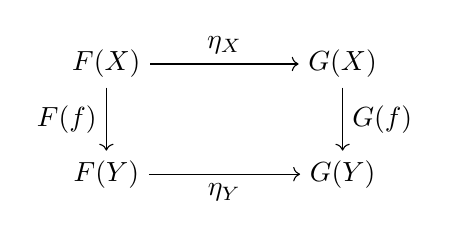
\begin{tikzpicture}[baseline=(current bounding box.center)]
\node (FX) at (0,0) {$F(X)$};
\node (GX) at (3,0) {$G(X)$};
\node (FY) at (0,-1.4) {$F(Y)$};
\node (GY) at (3,-1.4) {$G(Y)$};
\draw[->] (FX) -- node[above] {$\eta_X$} (GX);
\draw[->] (FY) -- node[below] {$\eta_Y$} (GY);
\draw[->] (FX) -- node[left] {$F(f)$} (FY);
\draw[->] (GX) -- node[right] {$G(f)$} (GY);
\end{tikzpicture}
\]
commutes for all morphisms $f : X \to Y$.

Intuition:
\begin{itemize}
    \item Naturality means: \emph{"attest first then transform" =
          "transform first then attest"}. 
    \item This is exactly the coherence needed for CEP attestation chains.
\end{itemize}

% ------------------------------------------------------------
\subsection*{A.4 Monoidal Categories}
% ------------------------------------------------------------

A \emph{monoidal category} is a category equipped with:
\begin{itemize}
    \item a tensor product $\otimes$ combining objects,
    \item a unit object $I$,
    \item coherence laws ensuring associativity and proper unit behavior.
\end{itemize}

In CEP, the relevant monoidal structure is \textbf{string concatenation}:
\begin{itemize}
    \item canonical components (name, address, date) combine via $\otimes$,
    \item the canonicalization functor preserves this structure strictly.
\end{itemize}

This allows the SNFEI to be treated as a universal construction.

% ------------------------------------------------------------
\subsection*{A.5 Oplax Functors}
% ------------------------------------------------------------

Given monoidal categories $(\mathbf{C}, \otimes)$ and $(\mathbf{D}, \otimes)$,
an \emph{oplax monoidal functor} $F : \mathbf{C} \to \mathbf{D}$ comes with
coherence maps
\[
F(X) \otimes F(Y) \to F(X \otimes Y)
\]
that need not be invertible.

Intuition:
\begin{itemize}
    \item Oplax functors allow \textbf{structure weakening}.
    \item This directly models jurisdictional adapters:
          some structure from the local schema may be incomplete or
          only partially mappable to the global vocabulary.
\end{itemize}

% ------------------------------------------------------------
\subsection*{A.6 Indexed Families and Fibrations}
% ------------------------------------------------------------

A \emph{fibration} $\pi : \mathbf{E} \to \mathbf{B}$ consists of:
\begin{itemize}
    \item a base category $\mathbf{B}$,
    \item a total category $\mathbf{E}$,
    \item a projection functor $\pi$,
    \item satisfying certain lifting properties.
\end{itemize}

The fiber over $B \in \mathbf{B}$ is the category
\[
\mathbf{E}_B = \{ E \in \mathbf{E} \mid \pi(E) = B \}.
\]

Intuition for CEP:
\begin{itemize}
    \item $\mathbf{B} = \mathbf{CEP}$ (identity-bearing records),
    \item $\mathbf{E} = \mathbf{CT}$ (records plus context tags),
    \item the fiber over $R$ is the set of all allowed context tags for $R$,
    \item fibers reindex naturally when $R$ evolves.
\end{itemize}

This formalizes the idea that context tags do not affect identity.

% ------------------------------------------------------------
\subsection*{A.7 Universal Properties (Informal)}
% ------------------------------------------------------------

A universal property specifies an object uniquely up to isomorphism
by the role it plays in relation to others.

In CEP:
\begin{itemize}
    \item the canonical string is universal for its admissible class
          of normalized components,
    \item the SNFEI is obtained by applying a hashing endofunctor,
    \item identity preservation follows from the uniqueness of the
          universal construction.
\end{itemize}

\bigskip
This concludes the appendix. Readers seeking more detail may consult
Mac~Lane~\cite{maclane1971categories},
Awodey~\cite{awodey2010category},
and Spivak~\cite{spivak2014category}.
   % Worked examples
% !TeX root = 00P3_cee_verticals.tex
\section*{Appendix B. Worked Examples}
\label{app:B}
\addcontentsline{toc}{section}{Appendix B. Worked Examples}

This appendix presents two concrete worked examples of bicategorical
interpretation: one for SME-friendly procurement and one for community
asset access.

\subsection*{B.1 SME-Friendly Procurement}

Consider a procurement lot with noisy inputs:
multiple spellings of the supplier's name,
ambiguous CPV codes,
and missing procedure-type metadata.

\paragraph{Step 1: Canonicalization (CEP base).}
\begin{enumerate}
  \item Normalize the entity fields (legal name, jurisdiction, value).
  \item Produce a canonical string in fixed order.
  \item Compute SNFEI via SHA-256.
\end{enumerate}

\paragraph{Step 2: Adapter semantics.}
Jurisdictional quirks (missing CPV codes, inconsistent currencies)
are handled via oplax functorial rules.

\paragraph{Step 3: CEE explanation.}
Evidence: low estimated value, open procedure type, minimal documentation.
Attribution: rule-based model ``sme-rule-v1''.
Narrative: ``This lot appears SME-friendly because \dots''.

Here the explanation is a 2-morphism refining the procurement relationship.

\subsection*{B.2 Community Asset Access}

Consider a neighborhood polygon and a dataset of parks and libraries.

Step 1: Construct CEP entities:
\begin{itemize}
  \item area entity (neighborhood),
  \item asset entities (parks, libraries),
  \item relationships linking assets to areas.
\end{itemize}

Step 2: Compute evidence layers and metrics:
population-served,
distance-to-assets,
equity index.

Step 3: Perform CEE prioritization:
Based on computed metrics and attribution model,
the vertical outputs a bundle with AREA\_ACCESS\_PRIORITY.
This bundle is a 2-morphism living above the area's incoming and
outgoing relationships.

\subsection*{B.3 Composition Across Verticals}

A municipality appearing in both verticals
supports functorial maps aligning their CEP entities and enabling
interoperable explanations.

   % Diagrammatic intuition
% !TeX root = 00P1_cae_ontology.tex

\clearpage
\section*{Appendix C. Glossary of Terms}
\addcontentsline{toc}{section}{Appendix C. Glossary of Terms}



This appendix provides concise definitions of key terms used throughout the paper.

\subsection*{Entity Kinds}

\textbf{Actor (A):}
An entity capable of bearing rights, obligations, or responsibilities within
civic systems when acting as an accountable party.
Examples include governments, public agencies, businesses, nonprofits, and universities.

\textbf{Site/Asset (S):}
A physical or operational entity that is acted upon but does not bear obligations.
Examples include facilities, buildings, infrastructure, and power plants.

\textbf{Instrument (I):}
An enduring construct that creates, modifies, or constrains rights, obligations,
or authority.
Examples include statutes, regulations, contracts, grants, permits, and licenses.

\textbf{Event (E):}
A time-indexed occurrence asserted under the authority of an Instrument.
Examples include payments, inspections, filings, violations, and audits.

\textbf{Jurisdiction (J):}
An entity that scopes authority, applicability, and governance, defining where
Instruments apply and where Events occur.
Examples include nations, states, municipalities, and regulatory regions.

\textbf{Observation (O):}
A measurement or indicator describing state, performance, or outcomes.
Observations do not create obligations or authorize actions.
Examples include health outcomes, coverage rates, emissions intensity measures,
and educational attainment indicators.

\subsection*{Design Concepts}

\textbf{Accountability Analysis:}
The examination of relationships, obligations, and authority structures within
civic systems in order to make responsibility and oversight inspectable.

\textbf{Accountability-bearing Relationship:}
A relationship that establishes or reflects accountability obligations between
entities, such as delegation of authority, participation in an Event, or the
measurement of outcomes.

\textbf{Applied Ontology:}
The use of ontological methods and principles to structure, clarify, and analyze
real-world domains for practical purposes.

\textbf{Competency Questions:}
Questions that an ontology should be able to answer, used to guide its development
and to evaluate its adequacy for the intended domain.

\textbf{Completeness:}
The extent to which an ontology captures the concepts and relationships required
for its stated purpose, without implying exhaustive coverage of all possible phenomena.

\textbf{Disjointness:}
The property that entity kinds do not overlap;
each entity belongs to exactly one kind.

\textbf{Domain Ontology:}
An ontology that captures concepts and relationships specific to a particular
application domain.
CAE is not a domain ontology.

\textbf{Domain-Constrained Reference Ontology:}
An ontology that provides a stable, reusable set of entity kinds and relationships
tailored to a particular domain, without committing to sector-specific taxonomies.
CAE is a domain-constrained reference ontology.

\textbf{Enduring Entity:}
An entity that persists through time while maintaining its identity, even as its
properties or relationships change.

\textbf{Entity Kind:}
A fundamental category of entities within the ontology, defined by distinct
identity criteria and invariant over time.

\textbf{Longitudinal Change:}
Variation or trends in data, conditions, or outcomes observed over extended periods
of time.

\textbf{Knowledge Representation:}
The formal specification of entities, relationships, and structures within a domain
to support interoperability and structured analysis.

\textbf{Ontology:}
A formal representation of entities within a domain
and the relationships that hold between them.

\textbf{Ontology Drift:}
The gradual divergence of an ontology's scope, structure, or commitments
from its original design intent.

\textbf{Selective Modeling:}
The inclusion of entities based on operational relevance rather than exhaustive
enumeration, introducing entities only when they participate in
accountability-bearing relationships.

\textbf{Semantics:}
The interpretation of structures and relationships defined by an ontology, without
implying evaluative or causal claims at the ontological level.

\textbf{Soundness:}
The property that an ontology's definitions and constraints are internally
consistent and aligned with their intended interpretations.

\textbf{Subclassing:}
The creation of a hierarchy of classes or categories within an ontology,
where more specific classes inherit properties and relationships from more
general ones.
CEA avoids subclassing within its six entity kinds.

\textbf{Time-Indexed Entity:}
An entity whose identity or assertions are associated with specific points or
intervals in time.

\textbf{Upper Ontology:}
A domain-independent ontology intended to provide general categories applicable
across many domains.
CAE is not an upper ontology.

\subsection*{Instrument Roles (Descriptive)}

\textbf{Normative role (descriptive):}
A functional role in which an Instrument establishes authority or defines
obligations.
Examples include statutes, acts, and treaties.

\textbf{Regulatory role (descriptive):}
A functional role in which an Instrument specifies procedures, thresholds, or
requirements.
Examples include regulations, rules, and administrative codes.


\subsection*{Methodological Context}

CAE is a formal ontology in the knowledge representation tradition:
a specification of what kinds of entities exist in the civic accountability domain,
what properties they have, and what relationships hold between them.
The six entity kinds form a strict partition: each entity belongs to exactly one
kind, and kinds do not overlap.
This structure supports rigorous, neutral reasoning about obligations, authority,
and evidence without embedding causal or evaluative assumptions.
   % Glossary of CAE terms (not category theory)

\bibliographystyle{plainnat}
\bibliography{bib_shared}
\end{document}